%%%%%%%%%%%%%%%%%%%%%%%%%%%%%%%%%%%%%%%%%%%%%%%%%%%%%%%%%%%%%%%%%%%%%%
% Template para artigos da SBC
% Adaptado para o trabalho prático de Processamento de Dados com Grafos
%%%%%%%%%%%%%%%%%%%%%%%%%%%%%%%%%%%%%%%%%%%%%%%%%%%%%%%%%%%%%%%%%%%%%%

\documentclass[12pt]{article}

\usepackage{sbc-template}
\usepackage{graphicx,url}
\usepackage[utf8]{inputenc}  
\usepackage{amsmath} % Para ambientes matemáticos
\usepackage{listings} % Para blocos de código
\usepackage{xcolor} % Para cores no código

% Configuração para blocos de código
\definecolor{codegreen}{rgb}{0,0.6,0}
\definecolor{codegray}{rgb}{0.5,0.5,0.5}
\definecolor{codepurple}{rgb}{0.58,0,0.82}
\definecolor{backcolour}{rgb}{0.95,0.95,0.92}

\lstdefinestyle{customStyle}{
    backgroundcolor=\color{backcolour},   
    commentstyle=\color{codegreen},
    keywordstyle=\color{magenta},
    numberstyle=\tiny\color{codegray},
    stringstyle=\color{codepurple},
    basicstyle=\ttfamily\footnotesize,
    breakatwhitespace=false,         
    breaklines=true,                 
    captionpos=b,                    
    keepspaces=true,                 
    numbers=left,                    
    numbersep=5pt,                  
    showspaces=false,                
    showstringspaces=false,
    showtabs=false,                  
    tabsize=2
}
\lstset{style=customStyle}
     
\sloppy

\title{Gestão de Dependências em Projetos Go com Ordenação Topológica}

% TODO: PREENCHER OS DADOS DOS AUTORES E INSTITUIÇÕES
\author{Nicholas Pereira Cristófaro\inst{1}, Nome Sobrenome do Aluno 2\inst{1}}

\address{Pontifícia Universidade Católica de Minas Gerais\\
  Belo Horizonte -- Minas Gerais -- Brasil
  \email{nicholaspcr@gmail.com, email2@dominio.com}
}

\begin{document} 

\maketitle

\begin{resumo} 
  A complexidade crescente dos sistemas de software modernos exige mecanismos robustos para a gestão de dependências. Este artigo apresenta o desenvolvimento de uma ferramenta para análise e visualização de dependências em projetos na linguagem Go. O problema da ordem de inicialização de pacotes é modelado como um grafo direcionado, onde os pacotes são os vértices e as importações representam as arestas. Utilizando o algoritmo de Kahn para ordenação topológica, a ferramenta determina a sequência de compilação segura e identifica a existência de dependências cíclicas, um erro crítico em Go. O trabalho detalha a implementação em Python, desde a análise do código-fonte até a geração de uma visualização gráfica interativa do grafo, alinhando-se ao tema de gestão de conflitos em sistemas de dependência.
\end{resumo}

\begin{abstract}
  The growing complexity of modern software systems demands robust mechanisms for dependency management. This paper presents the development of a tool for analyzing and visualizing dependencies in projects written in the Go language. The package initialization order problem is modeled as a directed graph, where packages are vertices and imports represent edges. Using Kahn's algorithm for topological sorting, the tool determines the safe compilation sequence and identifies the existence of cyclic dependencies, a critical error in Go. The work details the Python implementation, from source code parsing to the generation of an interactive graphical visualization of the graph, aligning with the theme of conflict management in dependency systems.
\end{abstract}


\section{Introdução}

O desenvolvimento de software contemporâneo é caracterizado pela modularidade e reutilização de código, resultando em sistemas compostos por um grande número de componentes interdependentes. A gestão dessa rede de dependências é um desafio central na engenharia de software. Falhas nesse gerenciamento podem levar a erros de compilação, comportamento inesperado em tempo de execução e dificuldades na manutenção e evolução dos projetos.

A linguagem de programação Go (Golang), desenvolvida pelo Google, possui um sistema de pacotes estático e um compilador que impõem regras estritas sobre as dependências. Uma dessas regras é que as dependências de um pacote devem ser inicializadas antes do próprio pacote. Isso garante a execução correta das funções `init()`, que são utilizadas para configurar o estado inicial de cada pacote. Quando um projeto contém uma dependência cíclica (por exemplo, pacote A importa B e pacote B importa A), o compilador Go gera um erro, pois não é possível determinar uma ordem de inicialização válida.

A ordem de inicialização de pacotes em Go pode ser modelada de forma natural como um grafo de dependências direcionado acíclico (DAG). Neste modelo, cada pacote é um vértice e uma diretiva `import` de um pacote A para um pacote B cria uma aresta direcionada de B para A, significando que A depende de B. A solução para determinar a sequência correta de inicialização é, portanto, encontrar uma ordenação topológica desse grafo.

Este trabalho se enquadra na proposta de "Gestão de Conflitos em Sistemas de Dependência", focando na modelagem, detecção de ciclos e execução segura baseada em ordenação topológica. Para isso, foi desenvolvida uma ferramenta em Python que:
\begin{itemize}
    \item Analisa recursivamente os arquivos de um projeto Go para extrair as relações de importação.
    \item Constrói um grafo de dependências direcionado a partir dessas relações.
    \item Aplica o algoritmo de Kahn para realizar a ordenação topológica dos pacotes.
    \item Gera uma visualização gráfica do grafo de dependências, destacando a ordem de inicialização em camadas.
\end{itemize}

O restante deste artigo está organizado da seguinte forma: a Seção 2 apresenta a fundamentação teórica sobre grafos, ordenação topológica e o sistema de pacotes do Go. A Seção 3 detalha a modelagem do problema e a arquitetura da ferramenta desenvolvida. A Seção 4 apresenta os experimentos realizados e discute os resultados obtidos. Finalmente, a Seção 5 conclui o trabalho e aponta direções para desenvolvimentos futuros.

\section{Fundamentação Teórica}
Esta seção aborda os conceitos fundamentais que sustentam o desenvolvimento deste trabalho, incluindo a teoria dos grafos, o algoritmo de ordenação topológica e as particularidades do sistema de pacotes da linguagem Go.

\subsection{Teoria dos Grafos}
Um grafo $G = (V, E)$ é uma estrutura matemática usada para modelar relações entre objetos. Consiste em um conjunto de vértices $V$ (ou nós) e um conjunto de arestas $E$ que conectam pares de vértices. Em um \textbf{grafo direcionado} (ou digrafo), as arestas têm uma direção, sendo representadas por pares ordenados de vértices $(u, v)$, indicando uma ligação de $u$ para $v$.

No contexto deste trabalho, o modelo utilizado é um grafo direcionado, onde:
\begin{itemize}
    \item \textbf{Vértices (V):} Representam os pacotes do projeto Go, tanto os locais (definidos no projeto) quanto os externos (bibliotecas padrão ou de terceiros).
    \item \textbf{Arestas (E):} Uma aresta direcionada $(u, v)$ existe se o pacote $v$ importa o pacote $u$. Isso significa que $u$ é uma dependência de $v$.
\end{itemize}

Uma métrica importante em grafos direcionados é o \textbf{grau de entrada (in-degree)} de um vértice, que corresponde ao número de arestas que chegam a ele. Um vértice com grau de entrada zero não possui dependências dentro do grafo.

\subsection{Ordenação Topológica}
A ordenação topológica de um grafo direcionado é uma ordenação linear de seus vértices tal que para toda aresta direcionada $(u, v)$, o vértice $u$ vem antes de $v$ na ordenação. Uma ordenação topológica só é possível se, e somente se, o grafo não contiver ciclos direcionados, ou seja, se for um \textbf{Grafo Acíclico Direcionado (DAG)}.

A existência de uma ordenação topológica no nosso grafo de dependências corresponde a uma sequência válida de inicialização dos pacotes Go. Se o grafo contiver um ciclo, não há ordenação topológica possível, o que corresponde a um erro de "dependência cíclica" no compilador Go.

\subsubsection{Algoritmo de Kahn}
Existem vários algoritmos para encontrar uma ordenação topológica. O escolhido para este trabalho foi o \textbf{algoritmo de Kahn}, devido à sua capacidade de processar os vértices em "camadas", o que é ideal para a visualização proposta. O algoritmo funciona da seguinte maneira:
\begin{enumerate}
    \item Calcular o grau de entrada (in-degree) de todos os vértices do grafo.
    \item Inicializar uma fila com todos os vértices que possuem grau de entrada igual a zero. Estes são os pacotes sem dependências.
    \item Enquanto a fila não estiver vazia:
    \begin{enumerate}
        \item Remover um vértice $n$ da fila e adicioná-lo à lista de ordenação topológica.
        \item Para cada vértice $m$ que é vizinho de $n$ (ou seja, para cada pacote que depende de $n$):
        \begin{enumerate}
            \item Decrementar o grau de entrada de $m$.
            \item Se o grau de entrada de $m$ se tornar zero, adicioná-lo à fila.
        \end{enumerate}
    \end{enumerate}
    \item Ao final, se o número de vértices na lista de ordenação topológica for igual ao número total de vértices do grafo, a ordenação foi bem-sucedida. Caso contrário, o grafo contém pelo menos um ciclo.
\end{enumerate}
A implementação deste algoritmo pode ser vista no arquivo `topological{\_}sorting.py`.

\subsection{Sistema de Pacotes e Módulos em Go}
Go organiza o código em pacotes, que são coleções de arquivos-fonte no mesmo diretório. O `go.mod` é um arquivo na raiz do projeto que define o caminho do módulo, que serve como um prefixo para todos os pacotes dentro do projeto, e também gerencia as dependências externas.

A diretiva `import` é usada para declarar dependências entre pacotes. Como mencionado, a ordem de execução das funções `init()` de cada pacote segue a ordem de dependência, exigindo uma resolução que é, na prática, uma ordenação topológica.

\section{Modelagem e Desenvolvimento da Ferramenta}
Esta seção descreve a arquitetura e os componentes da ferramenta desenvolvida, detalhando como o problema de análise de
dependências foi modelado e implementado em Python. A ferramenta é composta por três módulos principais, conforme os
arquivos `dependency{\_}graph{\_}builder.py`, `topological{\_}sorting.py` e `render.py`.

\subsection{Modelagem do Grafo de Dependências}
O problema foi modelado como um grafo direcionado $G = (V, E)$, conforme descrito na Seção 2.1. A estrutura de dados escolhida para representar o grafo foi um dicionário (hash map) em Python, onde as chaves são os nomes dos pacotes (vértices) e os valores são conjuntos contendo os pacotes que dependem deles (vizinhos).

\begin{itemize}
    \item \textbf{`graph = defaultdict(set)`:} Representa as arestas. `graph[u]` contém um conjunto de vértices `{v1, v2, ...}` para os quais existe uma aresta $(u, v1)$, $(u, v2)$, etc.
    \item \textbf{`in\_degree = defaultdict(int)`:} Armazena o grau de entrada de cada vértice, essencial para o algoritmo de Kahn.
\end{itemize}

\subsection{Componentes da Ferramenta}
A ferramenta segue um fluxo de execução claro: extração de dados, processamento (ordenação) e visualização.

\subsubsection{Extração e Construção do Grafo (\texttt{dependency\_graph\_builder.py})}
Este módulo é responsável por ler o sistema de arquivos e construir a representação do grafo. O processo é o seguinte:
\begin{enumerate}
    \item \textbf{Identificação do Módulo:} A classe `BuildDependencyGraph` inicia lendo o arquivo `go.mod` para determinar o prefixo do módulo do projeto. Isso é crucial para nomear corretamente os pacotes locais.
    \item \textbf{Busca por Arquivos Go:} O método `find\_go\_files` percorre recursivamente o diretório do projeto em
        busca de arquivos com a extensão `.go`, ignorando arquivos de teste (`\_test.go`).
    \item \textbf{Extração de Importações:} O método estático `extract\_imports` utiliza expressões regulares (regex) para analisar o conteúdo de cada arquivo Go e extrair todos os pacotes importados. Ele é projetado para lidar tanto com importações de linha única (`import "fmt"`) quanto com blocos de importação (`import (...)`).
    \item \textbf{Construção do Grafo:} O método `build\_dependency\_graph` orquestra o processo. Ele primeiro
        identifica todos os pacotes definidos localmente e depois itera sobre cada arquivo, usando as importações
        extraídas para construir o `graph` e popular o mapa `in\_degree`.
\end{enumerate}

\subsubsection{Ordenação Topológica e Detecção de Ciclos (\texttt{topological\_sorting.py})}
Este módulo implementa a lógica central do processamento.
\begin{itemize}
    \item \textbf{Detecção de Ciclos:} Antes de tentar a ordenação, o método `is\_cyclic` é chamado. Ele utiliza um algoritmo de busca em profundidade (DFS) para verificar a existência de ciclos no grafo. Se um ciclo é detectado, o programa informa o usuário e encerra, pois a ordenação topológica é impossível.
    \item \textbf{Ordenação com Algoritmo de Kahn:} O método `sort\_group` implementa o algoritmo de Kahn, conforme descrito na Seção 2.2.1. Em vez de retornar uma lista linear, nossa implementação retorna uma lista de listas (`list[list[str]]`), onde cada lista interna representa uma "camada" de pacotes que podem ser processados/compilados em paralelo, pois suas dependências da camada anterior já foram resolvidas.
\end{itemize}

\subsubsection{Visualização dos Resultados (\texttt{render.py})}
Para facilitar a compreensão da estrutura de dependências, um módulo de visualização foi criado utilizando a biblioteca `graphviz`.
\begin{enumerate}
    \item O grafo é renderizado como um `Digraph` com orientação da esquerda para a direita (`rankdir='LR'`).
    \item Os nós são agrupados em subgrafos com o mesmo `rank`, correspondendo às camadas calculadas pela função `sort\_group`. Isso alinha visualmente os pacotes que estão no mesmo nível da ordenação topológica.
    \item Os nós são coloridos de forma distinta: pacotes locais (parte do projeto analisado) têm uma cor, e pacotes externos (bibliotecas padrão ou de terceiros) têm outra. Isso ajuda a diferenciar o código do projeto de suas dependências externas.
    \item O resultado final é um arquivo SVG embutido em um HTML, que é automaticamente aberto no navegador, proporcionando uma visualização limpa e interativa.
\end{enumerate}

\begin{figure}[ht]
\centering
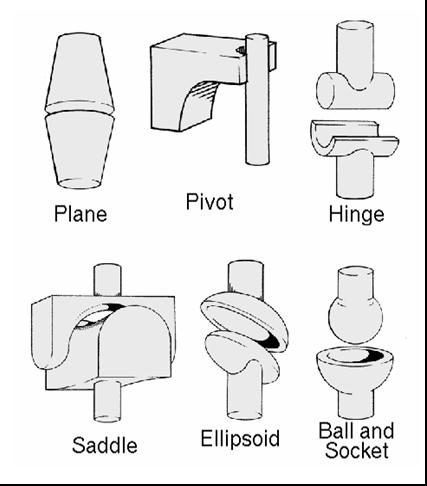
\includegraphics[width=.3\textwidth]{fig2.jpg}
\caption{Esta figura é um exemplo de uma legenda de figura que ocupa mais de uma
linha e é justificada considerando as margens mencionadas na Seção~\ref{sec:figs}.}
\label{fig:exampleFig2}
\end{figure}

Em tabelas, tente evitar o uso de fundos coloridos ou sombreados, e evite
linhas de enquadramento grossas, duplas ou desnecessárias. Ao relatar dados empíricos,
não use mais dígitos decimais do que o justificado por sua precisão e
reprodutibilidade. A legenda da tabela deve ser colocada antes da tabela (ver Tabela 1)
e a fonte usada também deve ser Helvetica, 10 pontos, negrito, com 6 pontos de
espaço antes e depois de cada legenda.

\begin{table}[ht]
\centering
\caption{Variáveis a serem consideradas na avaliação de técnicas de
interação}
\label{tab:exTable1}
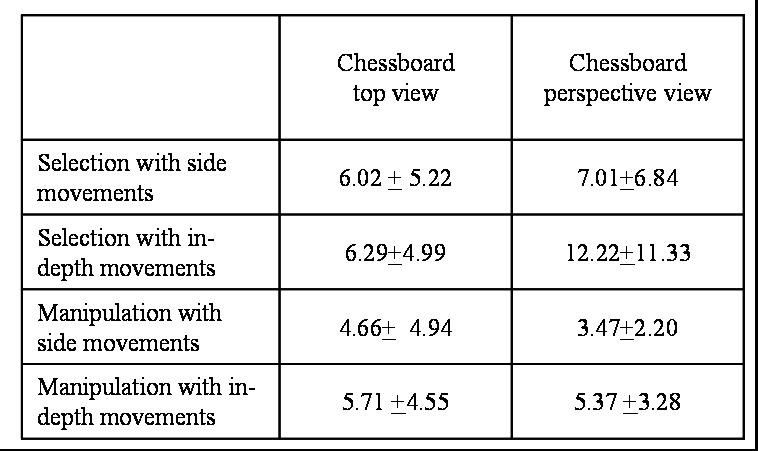
\includegraphics[width=.7\textwidth]{table.jpg}
\end{table}

\section{Imagens}

Todas as imagens e ilustrações devem ser em preto e branco, ou tons de cinza,
exceto para os artigos que estarão disponíveis eletronicamente (em CD-ROMs,
internet, etc.). A resolução da imagem no papel deve ser de cerca de 600 dpi para
imagens em preto e branco, e 150-300 dpi para imagens em tons de cinza. Não inclua
imagens com resolução excessiva, pois elas podem levar horas para imprimir, sem qualquer
diferença visível no resultado.

\section{Referências}

As referências bibliográficas devem ser inequívocas e uniformes. Recomendamos fornecer
as referências dos nomes dos autores entre colchetes, por exemplo, \cite{knuth:84},
\cite{boulic:91}, e \cite{smith:99}. As referências devem ser listadas usando fonte de tamanho 12, com 6 pontos de espaço
antes de cada referência. A primeira linha de cada referência não deve ser
recuada, enquanto as subsequentes devem ser recuadas em 0,5 cm.

\bibliographystyle{sbc}
\bibliography{sbc-template.bib}

\end{document}
